\section{Introduction}

A classification task can be seen as a sort of two-sample statistical test.
If a classifier trained over two samples can effectively distinguish between
them with better-than-chance performance, the classifier rejects the null
hypothesis that both samples come from the same distribution~\cite{friedman2004multivariate}.

While a formal statistical test can be more suitable when the alternative
hypothesis is known, machine learning classifiers can be a good alternative
when the data is complex and abundant~\cite{kirchler2020two,kim2021classification,pmlr-v119-liu20m}.

Furthermore, the representation ``learned'' by some classifiers can be helpful
to examine how the samples differ~\cite{friedman2004multivariate,lopez2016revisiting},
or it could be used later for other purposes, such as directly classifying future samples.

\medskip

\gls{SOM} is a technique for dimensionality
reduction. It is a type of neural network that learns a low-dimension representation
- generally 2D - of the original high-dimensional space while maintaining the topological
layout of the original data~\cite{kohonen1982self, Villmann1999}.

The learned map can be directly used for unsupervised clustering
and classification tasks if the training data is labeled~\cite{ultsch2005esom,ultsch2007emergence}.
Thus, \glspl{SOM} can be used as a building block of an ML-based two-sample test, similar to
\gls{kNN} or \emph{Neural Network} classifiers, with the valuable addition
of producing a representation that can be visualized.

In this chapter, we propose a multivariate statistical test based on
\glspl{SOM} that shows performance comparable to other techniques based on 
machine learning models and even superior for medium to big sample sizes. In addition to the 
$p$ value for $H_0: P = Q$, the test also outputs a trained \gls{SOM} model that can be of
use for other tasks, such as classification or visualization.
Our proposal uses a $\chi^2$ statistic to compare the densities of both samples on
the projected plane instead of relying on a training-testing split. This allows us to fully
utilize the sample data. To our knowledge, and based on the results from three
exhaustive surveys, using Self-Organizing Maps
to perform multidimensional two-sample testing has not been proposed
before~\cite{kaski1998bibliography,oja_bibliography_2003,polla_bibliography_2006}.

This statistical set can potentially be used with \PresQ to validate
high-dimensional \glspl{EDD}. The resulting projection can be used to identify objects
from multiple datasets that are co-located in the matched multidimensional space, satisfying
two of Borne's science requirements for data mining: \emph{Object Cross-Correlation} and
\emph{Nearest-neighbor identification}.

In section~\ref{sec:som_definitions}, we introduce classifier two-sample tests
and \glsxtrlong{SOM}. Then, in section~\ref{sec:som_chi2}, we describe our proposal
for a multidimensional non-parametric statistical test based on \glspl{SOM}.
In section~\ref{sec:som_exp_setup}, we describe the experimental setup we have used
to validate our proposal --- including the parametrization of the existing techniques
evaluated as a baseline ---. In section~\ref{sec:som_results}, we present the 
results.
Finally, in section~\ref{sec:som_conclusions}, we compile our conclusions and 
propose areas for future work.


\section{Definitions}
\label{sec:som_definitions}

\textbf{Classifier two-sample tests}
\label{sec:som_classifier2sample}
A binary classifier can be seen as a two-sample test. If a classifier has a better-than-chance
performance, it can be inferred that the two classes do not originate from the same underlying
population~\cite{friedman2004multivariate}. 

More formally, let $X = \{x_0,x_1,\ldots,x_n\}$  be a sample from $P$, and \linebreak
$Z = \{z_1,z_2,\ldots,z_m\}$ a sample from $Q$. A test statistic $\hat t \sim T$ is used to
``summarize'' the difference between both samples and, depending on a pre-established
significance level $\alpha$, used to reject the null hypothesis
$H_0: P = Q$ if $\alpha > P(T \ge \hat t | H_0)$.

When using a binary classifier for performing a statistical test, both samples are pooled
together $U = \{u_i\}_{i=1}^{n+m} = \{x_i\}_{i=1}^n \cup \{z_i\}_{i=1}^m$.
The samples originating from $P$ are labeled $y_i=1$, and the samples originating
from $Q$, $y_i=-1$.

The original proposal trains a classifier on the \emph{complete} pooled sample.
This classifier is then used to score each data point, generating a set of scores
for the first sample $S_+$ and for the second $S_-$. The multi-dimensional comparison
is thus reduced to a regular univariate two-sample test problem~\cite{friedman2004multivariate}.

Another approach is to split the pooled dataset $\{u_i\}_{i=1}^{n+m}$ into training
and testing sets. A classifier is then trained on the former, and the accuracy is
measured for the latter. The accuracy becomes the test statistic $\hat t$, which
follows asymptotically $N(\frac{1}{2}, \frac{1}{4 n_{test}})$~\cite{lopez2016revisiting}.
Alternatively, a permutation test can be used~\cite{kim2021classification}.
Two disadvantages of these kinds of tests are that they can not use the whole sample
for computing the test statistic --- therefore, they are not suitable for small
datasets --- and they are underpowered due to the discrete nature of the test
statistic~\cite{rosenblatt2021better}.

\textbf{\glsfmtlong{SOM}s}
is an unsupervised machine-learning algorithm that learns
a projection from a high-dimension input space into a low-dimension output space,
generally two-dimensional, to aid visualization.
The output space is modeled as a grid of \emph{neurons} --- a neural map ---
that \emph{responds} to a set of values from the input space~\cite{kohonen1982self}.
The output model preserves the topology of the input space: any continuous changes
in the input data cause a continuous change on the neural map~\cite{Villmann1999}.
In other words, input values close in the original high-dimensional space
trigger \emph{neurons} that are close in the low-dimensional projection~\cite{KOHONEN201352}.

The output space $W$ has to be defined before the training phase.
The user needs to define the shape of the grid --- square or hexagonal ---,
its size, and whether the map \emph{wraps around} (toroidal maps).
Each neuron $i$ from the model has an associated weight vector with the same
dimensionality as the input space, $w_{i}(t)$, where $t$ corresponds to the
\emph{epoch} of the training stage.
The initial values $w_i(t_0)$ can be assigned randomly or based on
Principal Component Analysis~\cite{KOHONEN201352}.

During the training, at each epoch $t$, each point $x$ from the training set
--- or a batch --- is mapped to its \gls{BMU}, which is
just the neuron whose weight vector is the closest given a distance metric $d$:

\begin{equation}
    \operatorname{bmu}(x) = \underset{w_i \in W}{\operatorname{argmin}} \; d(x, w_i)
\end{equation}

Once this is done, the \gls{BMU} and the weight of the neighboring neurons are updated, so they become closer to the input data point:

\begin{equation}
    w_i(t + 1) = w_i(t) + \alpha h_{i,b}(t) (x - w_b(t))
\end{equation}

Where $0 \le \alpha \le 1$ is a learning factor that may or may not depend on $t$,
and $0 \le h_{i,b} \le 1$ is the neighborhood function, with usually a Gaussian shape
that shrinks at each epoch~\cite{Villmann1999,wittek2013somoclu}.

\begin{equation}
    h_{i,b}(t) = \exp(- \frac{||w_i - w_b||}{\delta(t)})
\end{equation}

This process can be repeated for multiple epochs or until convergence.

\medskip

Thanks to the preservation of topology, \glspl{SOM} display emergent properties
when the grid is large enough: they can be directly used for clustering,
classification, and other machine learning techniques. These are referred as
\gls{ESOM}~\cite{ultsch2005esom}. This combination of emergence and
visualization capabilities motivates our proposal of a statistical test based
on \glspl{SOM}: a test that rejects the null hypothesis that two samples are equally distributed can also provide insights into how they differ.

\section{\texorpdfstring{$\chi^2$}{χ²} test on the projection over a \glsfmtlong{SOM}}
\label{sec:som_chi2}

Thanks to the topology preservation of \glspl{SOM}, a classifier can be trained
on the output space rather than the input space. For instance, for a \gls{kNN}
approach, neurons can be labeled using the training data and a majority rule. Later, test data
can be assigned the label from its \gls{BMU}. This is almost equivalent to a \gls{kNN} classifier with $k=1$.
Furthermore, neurons belonging to sparse regions can be left unlabeled, so test data projected
into them can be labeled as \emph{unknown class}~\cite{ultsch2005esom,silva2011som}.

While a \gls{SOM}-based classifier could be used in place of the neural or \gls{kNN} classifiers proposed
originally~\cite{lopez2016revisiting}, we propose a different approach that does not require
splitting the input data into training and testing sets, leveraging the distribution of the
data on the output space instead. The intuition behind is that if two samples are equally
distributed on the input space, they must be equally distributed on the output space.

More specifically, our method works as follows:

\begin{enumerate}
    \item We train a \gls{SOM} $M$ of size $(w, h)$ over $U = X \cup Z$
    \item We project $X$ and $Z$ separately over the \gls{SOM}  $M$
    \item We compute how many points from $X$ and how many from $Z$ are mapped to a given neuron $n_i$
\end{enumerate}

\begin{align}
    R_i = \sum_{x \in X} [ \operatorname{bmu}(x) = i ] && S_i = \sum_{z \in Z} [ \operatorname{bmu}(z) = i ]
\end{align}

\begin{enumerate}
    \setcounter{enumi}{3}
    \item Finally, we perform a a $\chi^2$ two sample test comparing the counts for both samples
    on the output space
\end{enumerate}

\begin{equation}
    \label{eq:chi2}
    \chi^2 = \sum_{i=1}^{w \times h}{ \left\{ \frac{(K_1 R_i - K_2 S_i)^2}{R_i + S_i} [ R_i + S_i > 0 ] \right\}}
\end{equation}

Where $K_1$ and $K_2$ are two constants used to adjust for different sample sizes:

\begin{align}
    \label{eq:k1k2} K_1 = \sqrt{\frac{|Y|}{|X|}} && K_2 = \sqrt{\frac{|X|}{|Y|}}
\end{align}

Note that we ignore the bins where there are 0 objects. Under the null hypothesis,
the test statistic $\chi^2$ follows a $\chi^2$
distribution with $k - c$ degrees of freedom, where $k$ is the number of cells
where ${R_i + S_i > 0}$, and $c = 1$ if the sample sizes are equal, or $c = 0$
otherwise~\cite{press1993numerical}.

As with any test based on binning, its main disadvantages are that its results may
depend on the binning (in this case, size of the \gls{SOM}) and that it requires
more data points.

On the other hand, since the \gls{SOM} adapts to the topology of the
original data, it is less susceptible to artifacts than a simple 2D histogram
due to the binning.

As with the classifier tests, as a side effect of the test, we are left with a
trained model that can be used for (1) visualization; and (2) for big enough
\gls{SOM}  and samples, even for clustering~\cite{ultsch2005esom}.

Unlike other classifier tests, with our proposal, the whole dataset can be used
for computing the statistic~\cite{kirchler2020two}. Additionally, thanks to the
regularization terms shown in equation \ref{eq:k1k2}, it also works with
unbalanced sample sizes, an advantage over most kernel-based methods~\cite{song2021fast}.

We have implemented our proposal using Somuclu, a parallel
tool for training self-organizing maps on large data sets~\cite{wittek2013somoclu}.

In the following section we describe the experimental setup used to
evaluate our proposal.
Later, in section~\ref{sec:som_results}, we report the results of our tests.

\section{Experimental setup}
\label{sec:som_exp_setup}

\subsection{Evaluated alternatives}

We have considered four different two-sample tests based on machine learning techniques.
All of them have in common the merging of both samples into a single set $Z$,
labeled with 1 if the sample comes from $X$ or -1 if comes from $Y$.

\textbf{Nearest neighbor type coincidences.}
The assumption under $H_0$ is that on the neighboring area of any point, the number of samples
belonging to $X$ and to $Y$ should be similar, while if $f \neq g$, then there will be areas with
a higher density of objects coming from one of the two sets~\cite{Henze1988,Schilling1986b}.

To perform the test, consider a neighbor $r$ of a sample $z_i \in Z$. We set

\begin{equation}
\begin{split}
    I_i(r) &= 1, \textrm{ if the label of } z_i \textrm{ and of } z_r \textrm{ match }\\
    I_i(r) &= 0, \textrm{otherwise}
\end{split}
\end{equation}

The statistical test:

\begin{equation}
    T_{n,k} = \sum_{i=0}^{n}\sum_{r=0}^{k} I_i(r)
\end{equation}

$n$ is the total number of samples, and $k$ the number of neighbors considered.
The distribution of the statistic is empirically obtained by applying a permutation test.
 
\textbf{Classifier two-sample tests.}
We have implemented the classifier two-sample test as described in section~\ref{sec:som_classifier2sample}
using \texttt{scikit-learn}~\cite{scikit-learn} neural
classifier\footnote{\texttt{sklearn.neural\_network.MLPClassifier}},
and \gls{kNN} classifier\footnote{\texttt{sklearn.neighbors.KNeighborsClassifier}}
with their default parameterization. Table~\ref{tab:classifier_diff} summarizes the differences with the original proposal. However, these differences should not significantly affect the performance~\cite{lopez2016revisiting}.

\begin{table}[htpb]
\centering
\begin{tabular}{lrr}
\multicolumn{1}{c}{\bfseries Parameter}       & \bfseries Revisiting\ldots & \texttt{scikit-learn}     \\ \hline
\multicolumn{3}{c}{\bfseries C2ST-NN} \\
Number of hidden layers &  1     &   1    \\
Number of neurons       & 20     & 100    \\
Activation              & ReLU   & ReLU   \\
Optimizer               & Adam   & Adam   \\
Epochs                  & 100    & 200    \\
\multicolumn{3}{c}{\bfseries C2ST-kNN} \\
$k$                     & $|X|/2$ & 5 \\
\end{tabular}
\caption[Differences between our parameterization]{
    Differences between our parameterization (\texttt{scikit-learn} defaults) and the one
    used in the original proposal~\cite{lopez2016revisiting}.
}
\label{tab:classifier_diff}
\end{table}

\textbf{Kernel Methods} are based on computing the \gls{MMD} between the samples,
which is the distance between their expected features in a Reproducing Kernel Hilbert Space.
In the original proposal~\cite{gretton2012kernel}, however, is computationally
expensive to compute the test statistic --- $O(N^2)$ --- and to approximate its distribution under
$H_0$ --- $O(N^2)$ or $O(N^3)$ depending on the method~\cite{zaremba2013b}.
A proposed alternative, MMD-B~\cite{zaremba2013b}, splits the input data into blocks, computes the original,
unbiased \gls{MMD} statistic on each block --- which are i.i.d ---, and averages the results.
Because of the central limit theorem, this average follows asymptotically a normal distribution.
Song \etal~\cite{song2021fast} propose another test statistic based on MMD-B that allows
unbalanced sample sizes and is more robust to the chosen kernel bandwidth (i.e., $\sigma$ on a Gaussian kernel).

\section{Results}
\label{sec:som_results}

We have performed five experiments to evaluate the performance of our \gls{SOM} 
two-sample test proposal.

For the first three setups - Normal, DC2, and the \emph{Open University Learning Analytics} dataset
- we set the significance level $\alpha = 0.1$. We then measure the run-time and empirical 
type I and type II error rates over $200$ repeated tests for all the evaluated
tests: (1) \gls{SOM}  (our proposal), (2) the \gls{kNN} permutation test~\cite{Schilling1986b},
and (3) two classifier tests (\gls{kNN} and Neural Network)~\cite{lopez2016revisiting}.
To obtain the $95\%$ confidence interval, we have used the Wilson score interval~\cite{Wilson1927}.

These values are measured for: (1) a fixed sample size of $n = m = 500$ and variable dimension;
and (2) for variable sample sizes and full dimensionality.

We have used a \emph{K-Best} feature selection to decide the order in which dimensions are added, from more to less informative.
Therefore, increasing the dimensionality is expected to have a diminishing return.

%%%%%%%%%%
% NORMAL %
%%%%%%%%%%
\subsection{Normal}
Figure~\ref{fig:normal_location} shows the error rates and run-time for a location
test of two multivariate Gaussian distributions with $D=1000$. For the first distribution,
all dimensions have a mean of $0$, while for the second one, all dimensions have a mean of $0$.

All tests can easily reject $H_0$ within a reasonable run-time. For
a high number of samples, however, the \gls{kNN} permutation test worsens its run-time performance,
probably due to the imbalance of the KD-Tree.

\begin{figure}[htpb]
    \centering
    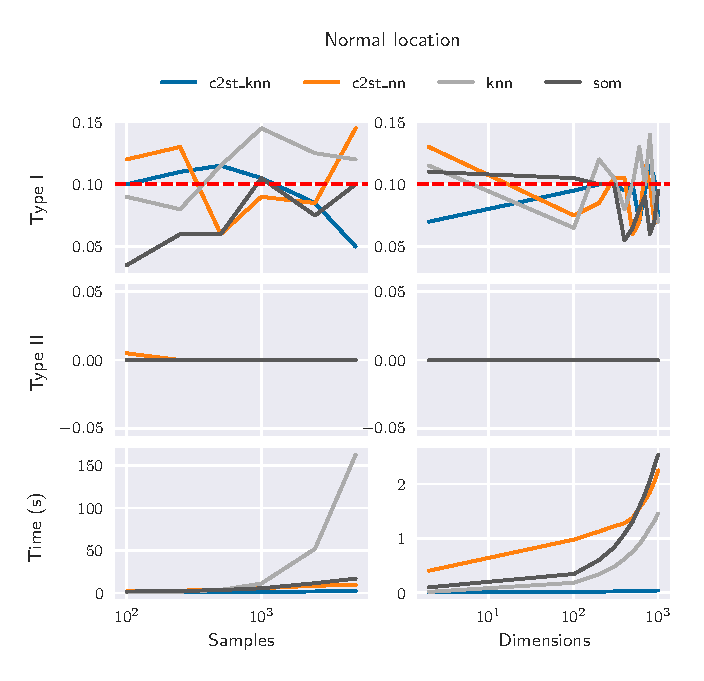
\includegraphics{images/6_som/normal_location}
    \caption[Location test for two multivariate Gaussian distributions.]{
    Location test for two multivariate Gaussian distributions with $D=1000$
    }
    \label{fig:normal_location}
\end{figure}

Figure~\ref{fig:normal_scale} shows the same variables for a scale test of two multivariate
Gaussian distributions with $D=1000$ and two random co-variances matrices samples from the
Wishart distribution~\cite{smith1972algorithm}. In this case, while the type I errors are
well bounded by the significance level, both algorithms based on neural networks
(C2ST-NN and \gls{SOM} ) require a higher number of samples to be able to reject $H_0$, with respect
to the other methods.

\begin{figure}[htbp]
    \centering
    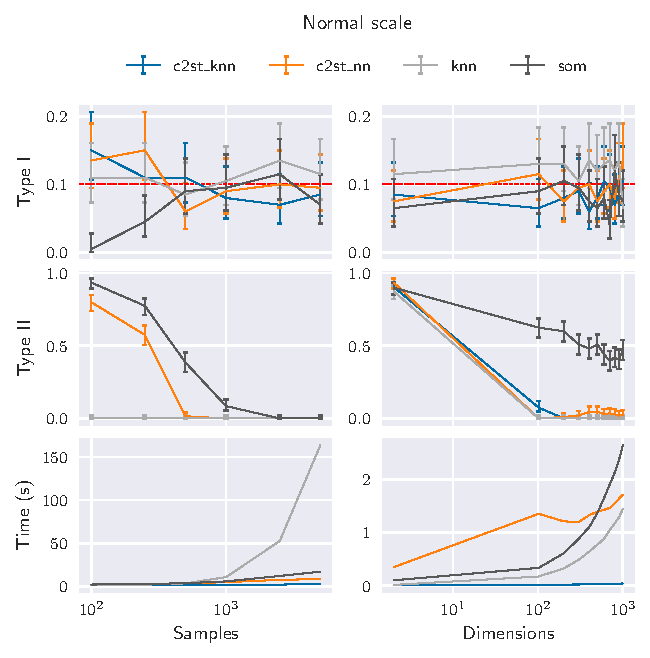
\includegraphics{images/6_som/normal_scale}
    \caption[Scale test for two multivariate Gaussian distributions.]{
    Scale test for two multivariate Gaussian distributions with $D=1000$}
    \label{fig:normal_scale}
\end{figure}

Ramdas \etal~\cite{ramdas2015decreasing} have argued that a ``fair'' evaluation of the
power of multivariate non-parametric tests as the dimensionality increases is to keep the
amount of information fixed. i.e. the \gls{KLD} between both distributions
should remain constant.

For the location test, this can be achieved by two multivariate Gaussians that only differ
on the first dimension, i.e. $(1, 0, \ldots, 0)$ vs $(0, 0, \ldots, 0)$.

For completeness, figure~\ref{fig:normal_fair_location} shows the performance of the classifier
two-sample tests being evaluated under this condition. We can see that they all fail to improve
their type II error as the dimensionality increase.

\begin{figure}[htbp]
    \centering
    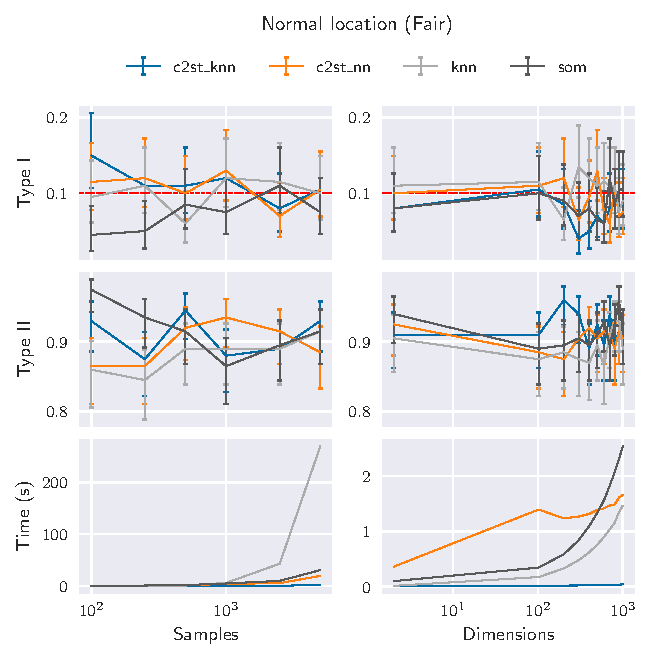
\includegraphics{images/6_som/normal_location_fair}
    \caption[Fair location test for two multivariate Gaussian distributions.]{
    Fair location test for two multivariate Gaussian distributions with $D=1000$}
    \label{fig:normal_fair_location}
\end{figure}

Finally, figure~\ref{fig:normal_fair_scale} shows the performance of the different
tests when only the scale of the first dimension differs, as Ramdas \etal propose
for a fair scale test. In this case, it is more evident that the type II error of all
tests worsens as the number of dimensions increases.

\begin{figure}[htbp]
    \centering
    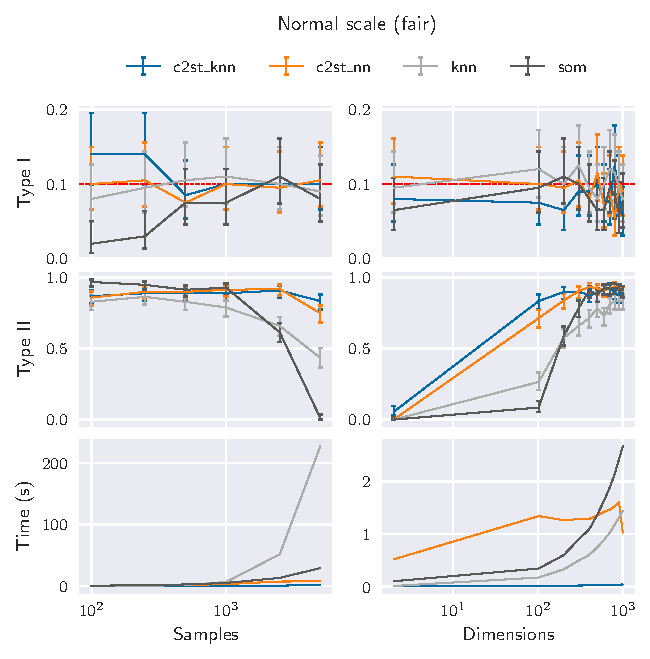
\includegraphics{images/6_som/normal_scale_fair}
    \caption[Fair scale test for two multivariate Gaussian distributions.]{
    Fair scale test for two multivariate Gaussian distributions with $D=1000$}
    \label{fig:normal_fair_scale}
\end{figure}

We consider that Ramdas \etal raise a valid point: given the same amount of available
information, additional dimensions do not help. However, for our \PresQ use case, this is an
unrealistic scenario: we are \emph{discovering} the matching dimensions, and each additional
feature will help discriminate whether two samples follow the same distribution.

%%%%%%%
% DC2 %
%%%%%%%
\subsection{DC2}
The datasets from this challenge come from a single catalog of astronomical
objects split based on the sky coordinates~\cite{EuclidDesprez2020}.

We generate three different samples:

\begin{enumerate}
    \item Samples from the full catalog
    \item Samples applying a magnitude cutout ($\text{MAG}_\text{VIS} < 22.)$
    \item Samples applying a \gls{SNR} cutout ($\text{VIS} / \text{VIS}_\text{Error} > 10.$)
\end{enumerate}

Following Ramdas' paper, in figure~\ref{fig:divergence_dc2}, we report
the estimated \gls{KLD} --- computed using a \gls{kNN} density estimation~\cite{perez2008kullback} --- between the datasets for an
increasing number of dimensions.
It can be seen that the amount of available information
rapidly increases for the magnitude cutout but barely for the \gls{SNR} filter,
probably because, for the latter, the means of the distributions do not change, only
their dispersion.

\begin{figure}[htbp]
    \begin{subfigure}[]{0.5\textwidth}
    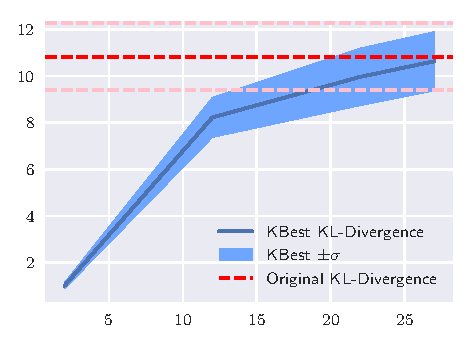
\includegraphics[width=\textwidth]{images/6_som/divergence/dc2_mag_divergence.eps}
    \caption{\gls{KLD} for the $\text{MAG}_\text{VIS}$ cutout}
    \end{subfigure}
    \hfill
    \begin{subfigure}[]{0.5\textwidth}
    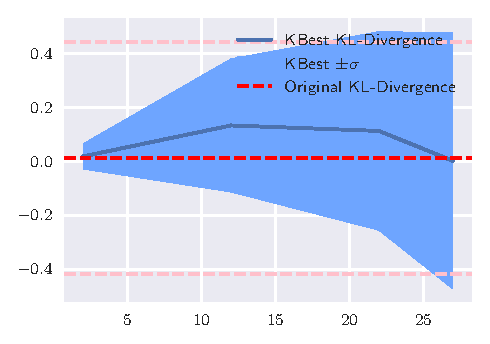
\includegraphics[width=\textwidth]{images/6_som/divergence/dc2_snr_divergence.eps}
    \caption{\gls{KLD} for the \gls{SNR} cutout}
    \end{subfigure}
    \caption{\glsfmtlong{KLD} for the DC2 samples. The original divergence
    corresponds to the original dimensionality of the dataset.}
    \label{fig:divergence_dc2}
\end{figure}

Figure~\ref{fig:dc2_mag} shows the measured performances for the DC2 with the magnitude
cutout. Even for a small sample size, the \gls{SOM}  test achieves very low type II errors, 
significantly better than the tests based on classifiers.
This may be because the \gls{SOM} and \gls{kNN}
tests can use the full sample, while the classifiers must split the data into training and testing sets.


\begin{figure}[htpb]
    \centering
    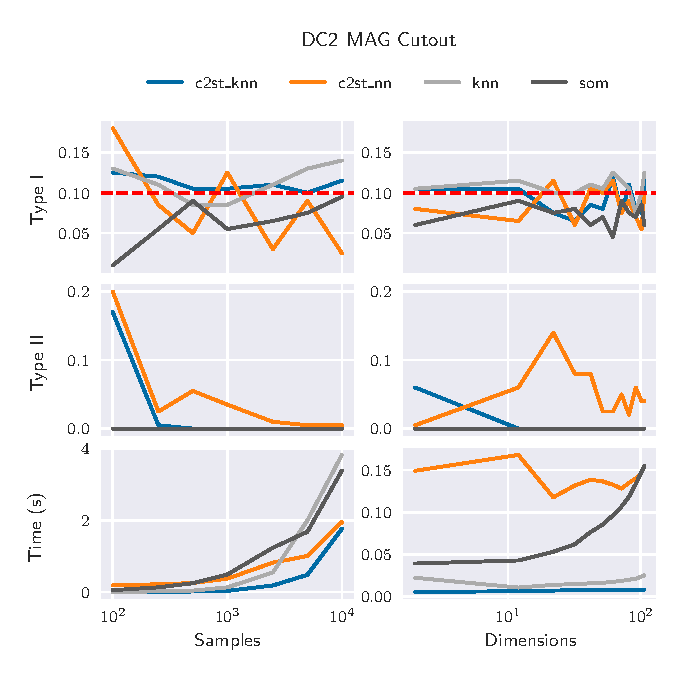
\includegraphics{images/6_som/dc2_mag}
    \caption[Statistical performance vs sample size and dimensionality.]{
    Statistical performance vs sample size (left) and dimensionality (right)}
    \label{fig:dc2_mag}
\end{figure}

Figure~\ref{fig:dc2_snr} shows the same performance metrics for the \gls{SNR} cutout.
In this case, as suggested by the \gls{KLD}, adding dimensions does not help any of the tests.
However, as the sample size increases, the \gls{kNN} and \gls{SOM}
tests improve their type II error rate. Bigger sample sizes do not help
the classifier-based tests.

\begin{figure}[htbp]
    \centering
    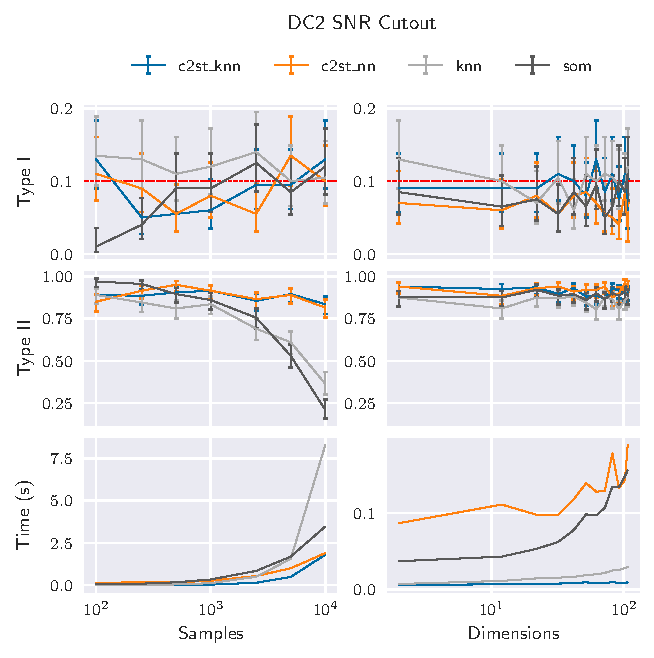
\includegraphics{images/6_som/dc2_snr}
    \caption[Statistical performance vs sample size and dimensionality.]{
    Statistical performance vs sample size (left) and dimensionality (right)}
    \label{fig:dc2_snr}
\end{figure}

\subsection{Open University Learning Analytics dataset}
\label{subsec:som_oulad}
The objective of this experiment is to prove that our proposed test can be successfully
used to test a hypothesis, providing an interpretable result useful for further
investigating the data.

We base our test on the \emph{Open University Learning Analytics}
dataset, which contains anonymized data about student demographics~\cite{kuzilek_open_2017}.

Let us consider the case of a researcher with the hypothesis that gender, age, and
region of origin influence a student's economic situation, or perhaps they could
be trying to deanonymize the data.

From this dataset, we can use the \gls{IMD} to measure poverty.
The null hypothesis $H_0$ would be that a sample from the overall population and a sample from
the poorest segment are indistinguishable, i.e., they come from the same distribution.

We take all students from the lower end of the poverty line and a sample of the same size
from the general population to test this hypothesis. We run the test using a \gls{SOM}  of size
$20\times20$. The null hypothesis is rejected with a p-value of $0$.

Unlike other statistical tests, in addition to the p-value, the researcher can use
the result of the \gls{SOM}  test to compare the projections of both samples.
Figure~\ref{fig:oulad_grid} shows the density of samples for each cell for the overall population
(left), the density of samples from the low-income students (center), and the relative difference
between both (right). The ``most different'' cells hint at how they are different.

\begin{figure}[t]
    \centering
    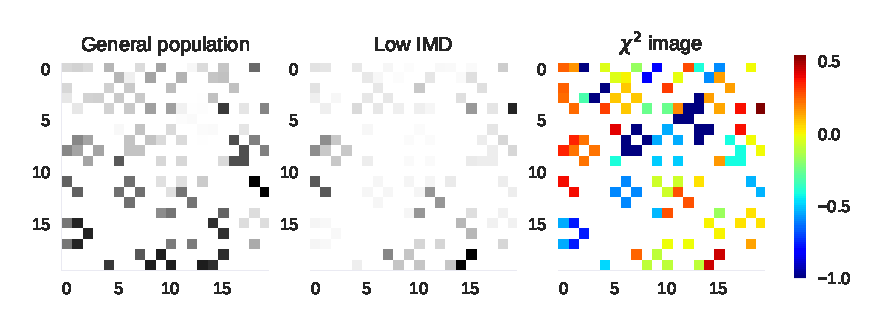
\includegraphics[width=\textwidth]{images/6_som/imd.eps}
    \caption[Comparing \glsfmtlong{SOM} density variations]{Density of samples for the general population (left), poorest segment (center) and
    relative difference (right). Cells with a value of $-1$ do not have any low-income students,
    while those with a value of $0.5$ show an ``excess'' with respect to the general
    population.}
    \label{fig:oulad_grid}
\end{figure}

If we pick one of the cells with the most significant bias towards low-income students,
we can see it contains only young female students from the \emph{North Western Region}.
In figure \ref{fig:oulad_hist}, we show the distribution of \gls{IMD} for the overall population (left)
and for this subset (right). Indeed, the income distribution for this demographics is
heavily skewed towards the low end. We could obtain this hindsight without prior knowledge of which
attributes correlate with the difference, only with the ``hunch'' that
there is a relation. Thus, we prove that our proposed test can be useful for data exploration.

\begin{figure}[htbp]
    \centering
    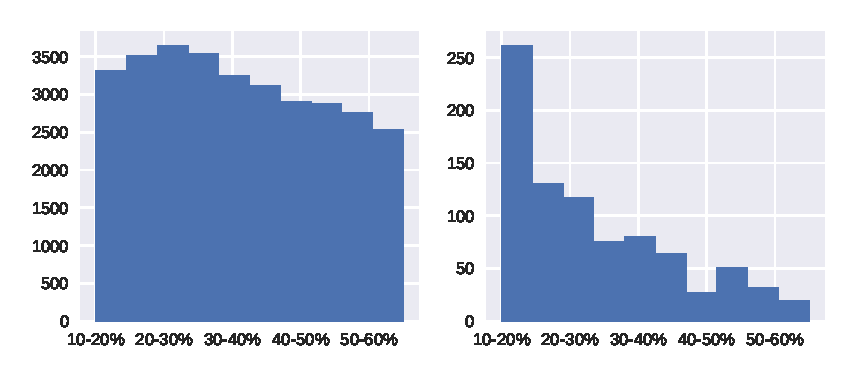
\includegraphics[width=\textwidth]{images/6_som/imd_histogram.eps}
    \caption[Histogram of the \glsfmtlong{IMD} for two populations]{
        \emph{Indices of Multiple Deprivations} for the general population (left) and for
        young female students from the \emph{North Western Region}.
    }
    \label{fig:oulad_hist}
\end{figure}

\subsection{Eye Movements}
\label{subsec:som_eye}
For generating this dataset, 11 subjects were shown a question and a list of ten 
associated sentences, of which one was the correct answer (C), four relevant (R), and five
irrelevant (I). Their eye movement was measured for each possible answer.
The overall measurements were summarized into 22 features, together with the
appropriate label for the sentence~\cite{salojarvi2005inferring}.

With this dataset, we aim to prove that our method can be competitive with other
start-of-the-art proposals, with the benefit of providing a trained model useful for
later purposes.

To evaluate the power of comparing different sets of measures, we replicate Song's
set up and run 2000 times\footnotemark the classifiers and \gls{SOM}  tests using a significance
level of $\alpha = 0.001$ for different sample sizes.
We report their statistical power in table \ref{tab:eye}.
The results from Song and MMD-B are extracted from Song's paper~\cite{song2021fast}.

\footnotetext{Song uses 1000 repetitions.}

\begin{table}[htbp]
    \centering
    \begin{tabular}{c r r r r r r}
        \hline
        \multicolumn{7}{c}{\thead{I vs. C}} \\
        \hline
        \thead{m = n} & \thead{Song} & \thead{MMD-B} & \thead{KNN} & \thead{C2ST-KNN} & \thead{C2ST-NN} & \thead{SOM} \\
        \hline
        100 & 0.826 & 0.374 & \textbf{0.973} & 0.164 & 0.079 & 0.042 \\
        200 & 0.998 & 0.850 & \textbf{1.000} & 0.565 & 0.349 & 0.947 \\
        300 & \textbf{1.000} & 0.985 & \textbf{1.000} & 0.863 & 0.644 & \textbf{1.000} \\
        400 & \textbf{1.000} & \textbf{1.000} & \textbf{1.000} & 0.968 & 0.882 & \textbf{1.000} \\
        \\
        \hline
        \multicolumn{7}{c}{\thead{R vs. C}} \\
        \hline
        \thead{m = n} & \thead{Song} & \thead{MMD-B} & \thead{KNN} & \thead{C2ST-KNN} & \thead{C2ST-NN} & \thead{SOM} \\
        \hline
        100 & 0.670 & 0.236 & \textbf{0.845} & 0.062 & 0.023 & 0.007 \\
        200 & 0.969 & 0.685 & \textbf{0.996} & 0.298 & 0.139 & 0.672 \\
        300 & 0.999 & 0.941 & \textbf{1.000} & 0.558 & 0.314 & 0.987 \\
        400 & \textbf{1.000} & 0.988 & \textbf{1.000} & 0.811 & 0.560 & \textbf{1.000} \\
    \end{tabular}
    \caption[Empirical statistical power for the eye movement datasets.]{
    Empirical statistical power for the eye movement datasets. We mark in
    bold the best results for each sample size.
    }
    \label{tab:eye}
\end{table}

The results show that our test has low power for small samples, but it rapidly gains
terrain compared to the classifier-based methods, being competitive even with 
kernel-based techniques. The nearest-neighbors method is remarkably efficient in all cases.

To evaluate the usefulness of the trained model obtained as part of running the
statistical test, we use the trained \glspl{SOM} as classifiers:
The neurons can be labeled according to the training data labels mapped into their
region using a majority rule. During classification, objects can be labeled according to the label of the neuron into which they are mapped. We performed a
50-fold cross-validation with a sample size of $n=m=409$, so each training set
has $n=m\approx 400$ elements for each label.

The obtained mean accuracy where: C vs. I 72.48\%; C vs. R 68.48\%; I vs. R 57.60\%.
Even with relatively small sample sizes, our results are comparable with those
reported on the paper from which the dataset was obtained:
65.8\% Correct vs. Incorrect (joint of Irrelevant and Relevant)~\cite{salojarvi2005inferring}.

Finally, as an exercise on interpretability, figure~\ref{fig:eye_distinct_features}
shows the value of the two most distinct code-book dimensions. These attributes,
related to the regression (re-reading a word) show a sharp distinction that
matches the distribution of samples from the Correct and Incorrect samples quite
well.
This matches the expectations from the original paper that regression features
indicate a high-level cognitive processing and,
therefore, correlate with conscious efforts when choosing a correct answer.

\begin{figure}[htb]
    \centering
    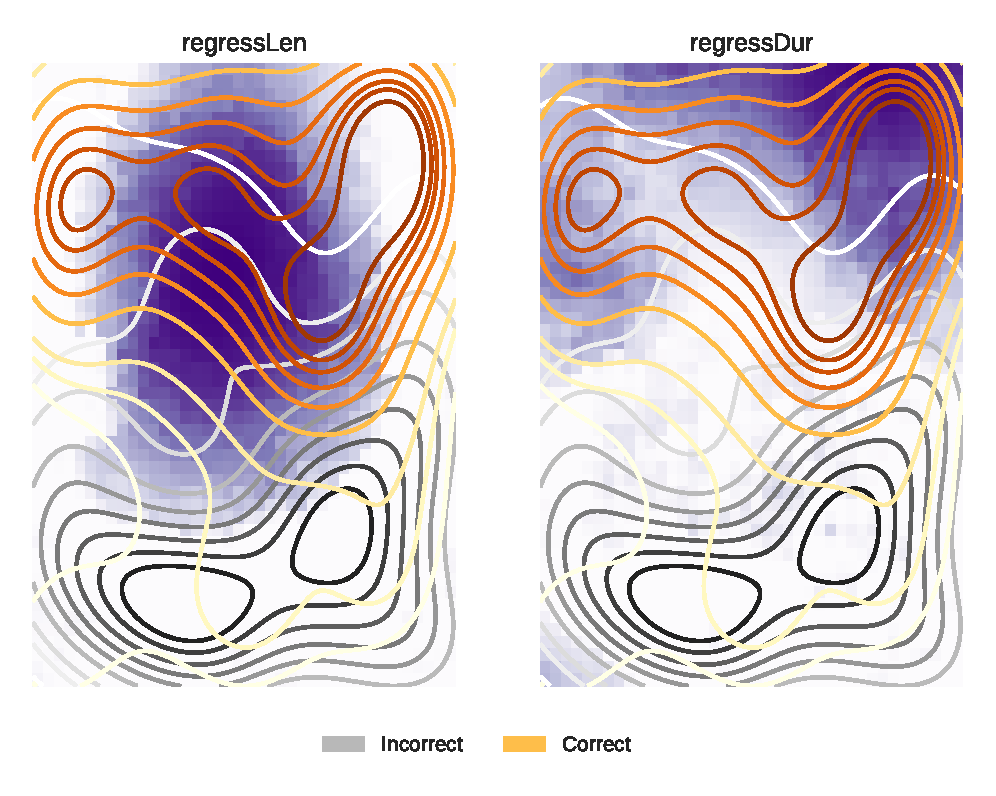
\includegraphics[width=\textwidth]{images/6_som/eye_regress.eps}
    \caption[Codebook values for the two most distinct features from the Eye dataset.]{
        Codebook values for the two most distinct features from the Eye dataset.
        Darker neurons are more sensitive to the given feature.
        The lines represent the density estimation for the Correct and \emph{Incorrect} samples
        over the \gls{SOM}.
        It is visible that the Incorrect category ``wraps'' around long regression distances, while the
        \emph{Correct} category correlates positively with the regression duration.
    }
    \label{fig:eye_distinct_features}
\end{figure}


\subsection{Age (IMDb Faces)}
The IMDb-WIKI dataset~\cite{rothe2018deep} contains 460,723 face images
extracted from IMDb. The authors additionally provide a neural network pre-trained
to predict the age of the face cutouts. Similarly to Song's experiments~\cite{song2021fast},
we have run the neural model over the IMDb faces, extracting the values from
the last hidden layer (4096 neurons) as the target multivariate distribution.

We then group the samples in age ranges and verify our proposal, comparing
500 samples from consecutive age groups, and repeat 500 times for each experiment. The
significance level is also set to $0.001$.

Table \ref{tab:age} shows the results for the \gls{SOM}  test, together
with the results reported by Song\etal for their kernel-based method and for
MMD-B\cite{zaremba2013b}.

\begin{table}[htbp]
    \centering
    \begin{tabular}{lrrrr}
    \hline
    Age ranges & \thead{Song} & \thead{MMD-B} & \thead{KNN} & \thead{SOM} \\
    \hline
    15-20 vs. 20-25 & 1.000 & 1.000 & 1.000 & 1.000 \\
    20-25 vs. 25-30 & 1.000 & 0.800 & 0.984 & 0.990 \\
    25-30 vs. 30-35 & 0.990 & 0.790 & 0.876 & 0.726 \\
    30-35 vs. 35-40 & 1.000 & 0.830 & 0.866 & 0.812 \\
    35-40 vs. 40-45 & 0.950 & 0.250 & 0.784 & 0.564 \\
    40-45 vs. 45-50 & 0.930 & 0.400 & 0.812 & 0.606 \\
    \hline
    \end{tabular}
    \caption{Statistical performances for the Age dataset}
    \label{tab:age}
\end{table}

For this particular experiment Song's proposal outperforms both MMD-B and the \gls{SOM} 
test, although our method comes second in statistical power.

%TODO: What about interpretability??

\subsection{\PresQ results}
As we have mentioned in the introduction, the motivating example is the unsupervised
discovery of shared attributes between multiple datasets using \PresQ (chapter~\ref{chapter:presq}),
obtaining, as a result, the list of sets of attributes and a trained model that can be used to
cross-match the datasets.

We have run two examples from the \PresQ paper using the proposed \gls{SOM}  based test
instead of the \gls{kNN} statistical test. For each of the examples, we measure:

\begin{description}
    \item[Ratio] of known shared attributes identified by \PresQ
    \item[Overhead] Number of tests per unique Equally-Distributed Dependency found
    \item[Time] that took \PresQ to finish, including the time taken for serializing the \gls{SOM}  models
\end{description}

Figure~\ref{fig:presq_som} reports the 95\% confidence interval ($\mu \pm 1.96 \sigma$)
for the \emph{relative differences} obtained when running with \gls{SOM}  vs
\gls{kNN}. Their distribution has been estimated using bootstrapping. The parametrization for
\PresQ was $\Lambda = 0.1$, $\gamma=0.95$, $\alpha=0.05$ and a sample size of 1000.

\begin{figure}[ht]
    \centering
    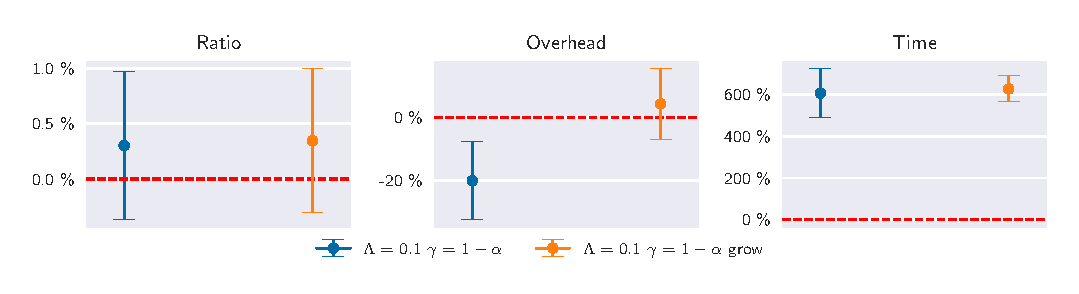
\includegraphics[width=\textwidth]{images/6_som/presq_som.eps}
    
    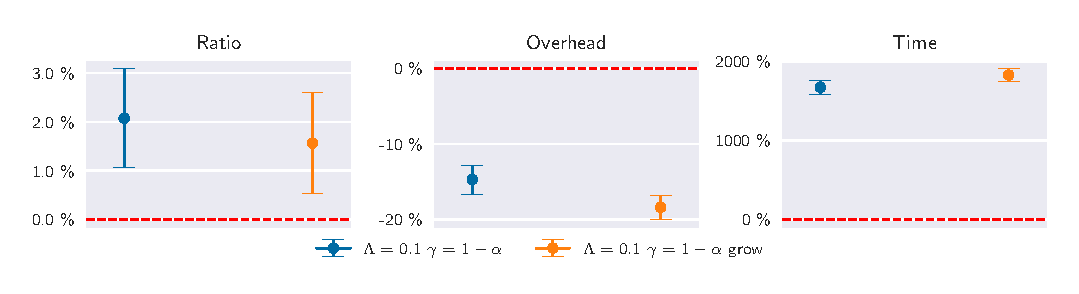
\includegraphics[width=\textwidth]{images/6_som/presq_som_aileron.eps}
    \caption[Relative difference between $\PresQ_{SOM}$ and $\PresQ_{kNN}$.]{
        Relative difference between $\PresQ_{SOM}$ and $\PresQ_{kNN}$.
        Top: DC2 dataset~\cite{EuclidDesprez2020}.
        Bottom: Ailerons / Elevators datasets~\cite{alcala2011keel}.
    }
    \label{fig:presq_som}
\end{figure}

The \gls{SOM}  test has a run-time penalty because it is a more complex model to train.
However, fewer tests are required for the same number of unique \gls{EDD} found. This is likely a consequence of
the \gls{kNN} test being slightly more prone to reject the equality of distribution than the \gls{SOM} 
test, as we can for instance see in figures \ref{fig:normal_location}, \ref{fig:normal_scale}.

\section{Conclusions}
\label{sec:som_conclusions}
As part of interactive data exploration, researchers may need to
compare multiple datasets.
These datasets can originate from multiple independent files or
generative models that need to be compared with reality. When these
datasets are of high dimensionality, and specially if the exploration is
tentative, developing tailored statistical tests can become impractical.
In those cases, relying on heuristic approaches based on machine
learning techniques, as classifiers, to decide whether two samples are
distinguishable becomes a good
alternative~\cite{friedman2004multivariate,kim2021classification}.

However, some of these methods, like neural networks, are hard to interpret
when rejecting the null hypothesis $H_0: P = Q$. In other words, they
reject that both samples originate from the same underlying distribution
but do not further assist the researcher.
Other models, such as random forests, are more  interpretable~\cite{friedman2004multivariate}.

In section~\ref{sec:som_chi2}, we have proposed another machine learning
technique based on \glsfmtlongpl{SOM}~\cite{kohonen1982self} that is
understandable and capable of pointing the researcher to where the differences
in a multidimensional space are. After all, \glspl{SOM} were initially
proposed as visualization aids. Nonetheless, they display interesting
emergent properties and can be used for clustering or classification as
well~\cite{ultsch2007emergence}.

In section~\ref{sec:som_results}, we have proven that the power of this
technique is comparable to other machine learning techniques and even
superior for medium-size datasets.
We have also proven in the experiment~\ref{subsec:som_oulad} that the
output can guide researchers toward refining a hypothesis. Thus, our
test can be a valuable asset to the researcher's tool-set, and complementary
to more formal hypothesis testing whenever considered necessary~\cite{rosenblatt2021better}.

For future work, it would be interesting to explore the possibilities of
properties of emergent Self-Organizing Maps to assist the researcher
in examining the differences.
For instance, clustering could help identify whole regions that differ
rather than focusing on individual neurons.
